\documentclass[a4paper, twocolumn, 12pt]{article}

\usepackage[english]{babel}

\usepackage{fullpage}
\usepackage{wallpaper}

\usepackage{graphicx}

\setlength{\columnsep}{1cm}

\usepackage{hyperref}

\pagestyle{empty}

\hypersetup{
    bookmarks=true,         % show bookmarks bar?
    unicode=false,          % non-Latin characters in Acrobat’s bookmarks
    pdftoolbar=true,        % show Acrobat’s toolbar?
    pdfmenubar=true,        % show Acrobat’s menu?
    pdffitwindow=false,     % window fit to page when opened
    pdfstartview={FitH},    % fits the width of the page to the window
    pdftitle={OpenEarth product sheet},    % title
    pdfauthor={Kees den Heijer},     % author
    pdfsubject={OpenEarth},   % subject of the document
    pdfcreator={Kees den Heijer},   % creator of the document
    pdfproducer={Kees den Heijer}, % producer of the document
    pdfkeywords={openearth} {data} {models} {tools}, % list of keywords
    pdfnewwindow=true,      % links in new PDF window
    colorlinks=true,       % false: boxed links; true: colored links
    linkcolor=blue,          % color of internal links (change box color with linkbordercolor)
    citecolor=blue,        % color of links to bibliography
    filecolor=blue,      % color of file links
    urlcolor=blue           % color of external links
}

\hyphenation{Open-Earth-Tools}


\begin{document}

\ThisULCornerWallPaper{.2}{figures/OpenEarth-logo-blurred-white-background.png}
 
\ThisURCornerWallPaper{.25}{figures/deltares_merk_pantone.pdf}

\section*{What is OpenEarth?}
\href{http://www.openearth.eu}{OpenEarth} is a free and open source initiative to deal with \href{https://publicwiki.deltares.nl/display/OET/Data}{Data}, \href{https://publicwiki.deltares.nl/display/OET/Models}{Models} and \href{https://publicwiki.deltares.nl/display/OET/Tools}{Tools} in earth science \& engineering projects, currently mainly marine \& coastal. In current practice, research, consultancy and construction projects commonly spend a significant part of their budget to setup some basic infrastructure for data and knowledge management. Most of these efforts disappear again once the project is finished. As an alternative to these ad-hoc approaches, \href{http://www.openearth.eu}{OpenEarth} aims for a more continuous approach to data \& knowledge management. It provides a platform to archive, host and disseminate high quality data, state-of-the-art model systems and well-tested tools for practical analysis. Through this project-superseding approach, marine \& coastal engineers and scientists can learn from experiences in previous projects and each other. This may lead to considerable efficiency gains, both in terms of budget and time. The following papers describe the \href{http://www.openearth.eu}{OpenEarth} approach in more detail: \href{https://www.iadc-dredging.com/ul/cms/terraetaqua/document/3/7/3/373/373/1/article-openeartha-knowledge-management-workflow-for-dredging-projects-terra-et-aqua-131-1.pdf}{Terra et Aqua, 2013}, \href{http://dx.doi.org/10.3990/2.177}{NCK 2012} \& \href{https://publicwiki.deltares.nl/download/attachments/42401895/VanKoningsveld\%20et\%20al.\%20\%28WODCON2010\%29\%20Data\%20\%20Models\%20and\%20Tools\%20-\%20V17.pdf?version=1&modificationDate=1287560844000&api=v2}{WODCON 2010}.
Within the \href{http://www.openearth.eu}{OpenEarth} community two types of users can be distinguished: 1) \href{https://publicwiki.deltares.nl/display/OET/OpenEarth#OpenEarth-OpenEarthusers}{\#OpenEarth users} and 2) \href{https://publicwiki.deltares.nl/display/OET/OpenEarth#OpenEarth-OpenEarthdevelopers}{\#OpenEarth developers}.


\begin{figure}[ht]

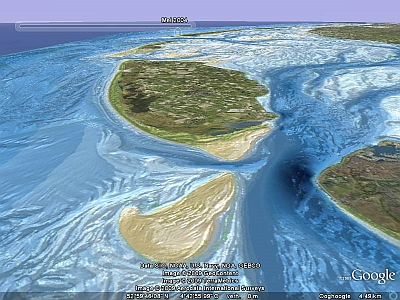
\includegraphics[width=\linewidth]{figures/vaklodingen_small.jpg}
\caption{Example of Google Earth visualization of bathymetry created with OpenEarthTools}
\end{figure}

\section*{OpenEarth users}
\href{http://www.openearth.eu}{OpenEarth} users are particularly interested in using data, models and tools that have become available through \href{http://www.openearth.eu}{OpenEarth} for project purposes. For these users easily installable software packages as well as user manuals and tutorials are available in the \href{https://publicwiki.deltares.nl/display/OET/OpenEarth+Product+Suite}{OpenEarth Product Suite}. An explanation on how to get access to data is given in the \href{https://publicwiki.deltares.nl/display/OET/Getting+started}{Getting started} section.
\section*{OpenEarth developers}
\href{http://www.openearth.eu}{OpenEarth} developers participate actively in the dissemination of new datasets and model systems and the development \& improvement of all kinds of handy tools. If you wanna be an \href{http://www.openearth.eu}{OpenEarth} developer, please follow this link to learn about the \href{https://publicwiki.deltares.nl/display/OET/OpenEarth+developer+in+five+easy+steps}{five easy steps to become an OpenEarth developer}.
\section*{About us}
\href{http://www.openearth.eu}{OpenEarth} is, among others, supported by the concerted effort of professionals from \href{http://www.deltares.nl}{Deltares} (formerly Delft Hydraulics), \href{http://www.tudelft.nl}{Delft University of Technology}'s \href{http://www.waterbouw.tudelft.nl/}{Hydraulic Engineering} and \href{http://www.fluidmechanics.tudelft.nl/}{Environmental Fluid Mechanics} sections, \href{http://www.vanoord.com/}{Van Oord Dredging and Marine Contractors}, \href{http://www.arcadis.nl}{Arcadis} and \href{http://www.unesco-ihe.org/}{UNESCO-IHE}. Please visit our \href{https://www.linkedin.com/groups?home=&gid=3746269&trk=anet_ug_hm}{OpenEarth LinkedIn group} to see the more than 400 members. More background information on \href{http://www.openearth.eu}{OpenEarth} can be found here.
\end{document}